\chapter{Variable Structure Models}
The composition of a variable structure model changes through time. New components are added as machinery is installed in a factory, organisms reproduce, or shells are fired from a cannon. Existing components are removed as machines break, organisms dies, or shells in flight find their targets. Components are rearranged as parts move through a manufacturing process, organisms migrate, or a command and control network loses communication lines. But structure change can not occur willy nilly if we want our simulation to produce well defined, repeatable outcomes. For this reason, \adevs\ provides a simple but effective mechanism for coordinating structure changes with model state transitions\footnote{The dynamic structure features in \adevs\ are based on the Dynamic DEVS modeling formalism described in A.M. Uhrmacher's paper ``Dynamic structures in modeling and simulation: a reflective approach", ACM Transactions on Modeling and Computer Simulation (TOMACS), Volume 11, Issue 2, pgs. 202-232, April 2001.}.

\section{Building and Simulating Variable Structure Models}
Every \adevs\ model, \classname{Network} and \classname{Atomic}, has an abstract method called \methodname{model\_transition}. This method is inherited from the \classname{Devs} class that is at the top of the \adevs\ class hierarchy. The signature of the \methodname{model\_transition} method is
\begin{verbatim}
bool model_transition()
\end{verbatim}
and its default implementation simply returns false.

At the end of every simulation cycle the simulator invokes the \methodname{model\_transition} method of every \classname{Atomic} model that changed in that cycle. When the \methodname{model\_transition} method is invoked the \classname{Atomic} model can do almost anything it likes except alter the component set of a \classname{Network} model.
If the \methodname{model\_transition} method returns true, then the simulator will also call the model's parent.
The parent is, of course, a \classname{Network} model; its \methodname{model\_transition} method may add, remove, and rearrange components. But it must not delete components! The simulator will automatically delete removed components when the structure change calculations are finished. As before, if the \classname{Network}'s \methodname{model\_transition} method returns true then the simulator will invoke the \methodname{model\_transition} method of the \classname{Network}'s parent.

After invoking every eligible model's \methodname{model\_transition} method, the simulator performs a somewhat complicated cleanup process. This process requires that simulator construct two sets. The first set contains all of the components that belonged to all of the \classname{Network} models whose \methodname{model\_transition} method was invoked and all of the components belonging to components that are in this set. The second set is defined in the same way, but it is computed using component sets as they exist after the \methodname{model\_transition} methods have been invoked. The simulator deletes every model that has actually been removed; these are the models in the first set but not in the second. The simulator initializes every model that is genuinely new by computing its next event time (i.e., its creation time plus its time advance) and putting it into the event schedule; these are the models in the second second set but not in the first. The simulator leaves all other models alone. This confusing procedure is illustrated in Fig. \ref{fig:set_defns}.
\begin{figure}[ht]
\centering
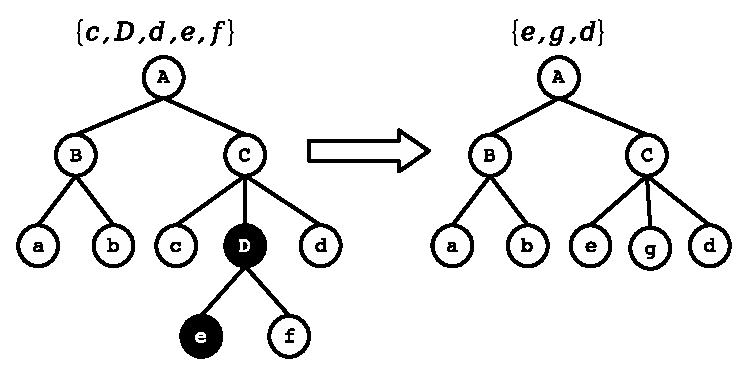
\epsfig{file=var_struct_models_figs/var_struct_model_sets.eps}
\caption{The black models' \methodname{model\_transition} methods returned true. The set of components considered before and after the structure change are shown in the before (left) and after (right) trees. The set of deleted components is $\{c,D,d,e,f\}-\{e,g,d\} = \{c,D,f\}$. The set of new components is $\{e,g,d\} - \{c,D,d,e,f\} = \{g\}$.}
\label{fig:set_defns}
\end{figure}

The \methodname{model\_transition} method can break the strict hierarchy and modularity that is usual observed when building \classname{Atomic} and \classname{Network} models. Any \classname{Network} model can modify the component set of any other model regardless of proximity or hierarchy. The potential for anarchy is great; the design of a variable structure model should be carefully considered. There are two approaches that are simple and, in many cases, entirely adequate.

The first approach is to allow only \classname{Network} models to effect structure changes and to restrict those changes to the \classname{Network}'s immediate sub-components. With this approach, an \classname{Atomic} model initiates a structure change by posting a structure change request for its parent \classname{Network}. The \classname{Atomic} model's \methodname{model\_transition} method then returns true causing its parent's \methodname{model\_transition} method to be invoked. The parent \classname{Network} model then retrieves and acts on the posted structure change request. The \classname{Network} repeats this process if it wants to effect structure changes involving models other than its immediate children.

The second approach allows arbitrary structure changes by forcing the model at the very top of the hierarchy to invoke its \methodname{model\_transition} method. This causes the simulator to consider every model in the aftermath of a structure change. As in the first approach, an \classname{Atomic} model that wants to effect a structure change uses its \methodname{model\_transition} method to post a change request for its parent. This is percolated up the model hierarchy by the \classname{Network} models whose \methodname{model\_transition} methods always return true. 

The first approach trades flexibility for execution time; the second approach trades execution time for flexibility. With the first approach, structure changes that involve a small number of components require a small amount of work by the simulator. With the second approach, every structure change requires the simulator to include every part of the model in its set calculations regardless of the structure change's actual extent, but the scope of a structure change is unlimited.

\section{A Variable Structure Example}
The Custom Widget Company is expanding its operations. Plans are being drawn for a new factory that will make custom gizmos (and the company name will be changed to The Custom Widget and Gizmo Company). The factory machines are expensive to operate. To keep costs down, the factory will operate just enough machinery to fill outstanding gizmo orders in sufficient time. The factory must have enough machinery to meet peak demand, but much of the machinery will be idle much of the time.
The factory engineers want to answer two questions: how many machines are needed and how much will it costs to operate the them. 

We are going to use a variable structure model to answer these two questions. The model will have three components: a generator that creates factory orders, a model of a single machine, and a model of the factory which contains the machine models and activates and deactivates machines as required to satisfy demand. The complete factory model is illustrated in Fig. \ref{fig:factory_model}.
\begin{figure}[ht]
\centering
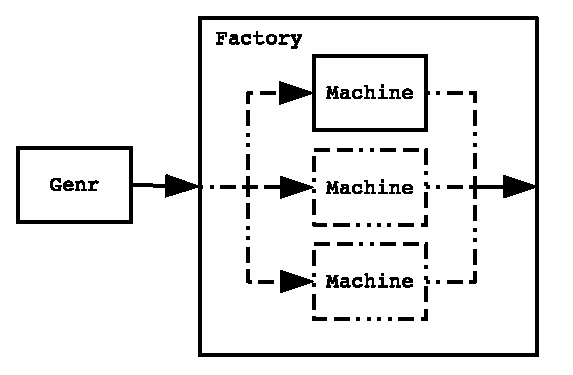
\epsfig{file=var_struct_models_figs/factory_block_diagram.eps}
\caption{Block diagram of the variable structure factory model. The broken lines indicate structural elements that are subject to dynamic changes.}
\label{fig:factory_model}
\end{figure}

The generator creates new orders for the factory. Each order is identified with its own integer label, and the generator produces orders at the rate anticipated by the factory planners. The order arrival rate and, consequently, the time advance of the generator are not constants. Demand at the factory is expected to be fairly steady with a new order arriving every 1/2 to 2 days; demand is modeled with a random variable uniformly distributed in the range [0.5,2]. Here is the generator code:
\begin{verbatim}
#include "adevs.h"
// The Genr models factory demand. It creates new orders every 0.5 to 2 days.
class Genr: public adevs::Atomic<int>
{
    public:
        /**
         * The generator requires a seed for the random number that determines
         * the time between new orders.
         */
        Genr(unsigned long seed):adevs::Atomic<int>(),next(1),u(seed){ set_time_to_order(); }
        // Internal transition updates the order counter and determines the next arrival time
        void delta_int() { next++; set_time_to_order(); }
        // Output function produces the next order
        void output_func(adevs::Bag<int>& yb) { yb.insert(next); }
        // Time advance returns the time until the next order
        double ta() { return time_to_order; }
        // Model is input free, so these methods are empty
        void delta_ext(double,const adevs::Bag<int>&){}
        void delta_conf(const adevs::Bag<int>&){}
        // No explicit memory management is needed
        void gc_output(adevs::Bag<int>&){}
    private:
        // Next order ID
        int next;
        // Time until that order arrives
        double time_to_order;
        // Random variable for producing order arrival times
        adevs::rv u;
        // Method to set the order time
        void set_time_to_order() { time_to_order = u.uniform(0.5,2.0); }
};
\end{verbatim} 

The machine model is similar to the \classname{Clerk} model that appeared in section \ref{chapter:intro}. Each machine requires 3 days make a gizmo and orders are processed first come first serve. The \classname{Machine}'s \methodname{model\_transition} method is inherited from the \classname{Atomic} class, which inherited it from the \classname{Devs} class (the inheritance hierarchy is \classname{Devs} $\leftarrow$ \classname{Atomic} \classname{Machine}). I'll discuss the role of the \methodname{model\_transition} method after introducing the \classname{Factory} class; here is the \classname{Machine} model code.
\begin{verbatim}
#include "adevs.h"
#include <cassert>
#include <deque>
/**
 * This class models a machine as a fifo queue and server with fixed service time.
 * The model_transition method is used, in conjunction with the Factory model_transition
 * method, to add and remove machines as needed to satisfy a 6 day turnaround time
 * for orders. 
 */
class Machine: public adevs::Atomic<int> 
{
    public:
        Machine():adevs::Atomic<int>(),tleft(DBL_MAX){}
        void delta_int()
        {
            q.pop_front(); // Remove the completed job
            if (q.empty()) tleft = DBL_MAX; // Is the Machine idle?
            else tleft = 3.0; // Or is it still working?
        }
        void delta_ext(double e, const adevs::Bag<int>& xb)
        {
            // Update the remaining time if the machine is working
            if (!q.empty()) tleft -= e;
            // Put new orders into the queue
            adevs::Bag<int>::const_iterator iter = xb.begin();
            for (; iter != xb.end(); iter++) 
            {
                // If the machine is idle then set the service time
                if (q.empty()) tleft = 3.0;
                // Put the order into the back of the queue
                q.push_back(*iter);
            }
        }
        void delta_conf(const adevs::Bag<int>& xb)
        {
            delta_int();
            delta_ext(0.0,xb);
        }
        void output_func(adevs::Bag<int>& yb)
        {
            // Expel the completed order
            yb.insert(q.front());
        }
        double ta()
        {
            return tleft;
        }
        // The model transition function returns true if another order can not
        // be accommodated or if the machine is idle.
        bool model_transition()
        {
            // Check that the queue size is legal
            assert(q.size() <= 2);
            // Return the idle or full status
            return (q.size() == 0 || q.size() == 2);
        }
        // Get the number of orders in the queue
        unsigned int getQueueSize() const { return q.size(); }
        // No garbage collection 
        void gc_output(adevs::Bag<int>&){}
    private:
        // Queue for orders that are waiting to be processed
        std::deque<int> q;
        // Time remaining on the order at the front of the queue
        double tleft; 
};
\end{verbatim}

The number of \classname{Machine} models in the \classname{Factory} any time is determined by the current demand for gizmos. The real factory, of course, will have a set number of physical machines on the factory floor, but the planners do not yet know how many machines are needed. A variable structure model that creates and destroys machines as needed is a good way to accommodate this uncertainty (a design decision similar to using a linked list in place of a fixed size array). 

The Custom Widget and Gizmo Company has built its reputation on a guaranteed service time, from order to delivery, of 15 days. This leaves only 6 days for the manufacturing process (the remaining time being consumed by order processing, delivery, etc.). 
A single machine can meet this schedule if it has at most one order waiting in its queue. But it costs a dollar a day to operate a machine and so the factory engineers want to minimize the number of machines working at any particular time. With this goal, the factory operating policy has two rules:
\begin{enumerate}
\item assign incoming orders to the active machine that can provide the shortest turn around time and
\item keep just enough active machines to have capacity for one additional order.
\end{enumerate}
The \classname{Factory} model implements this policy in the following way. When a \classname{Machine} becomes idle or its queue is full (i.e., the machine is working on one order and has another order waiting in its queue) then its \methodname{model\_transition} method returns true. This causes the \classname{Factory}'s \methodname{model\_transition} method to be invoked. The \classname{Factory} first looks for and removes machines that have no work and then examines each remaining machine to determine if the required one unit of additional capacity is available. If the required unit of additional capacity is not available then the \classname{Factory} creates a new machine.

This is an example of the first approach to building a variable structure model. With this design, the set calculations that are done when the \classname{Factory}'s \methodname{model\_transition} method is invoked are limited to instances where \classname{Machine} models are likely to be created or destroyed. Our design, however, is complicated somewhat by the need for \classname{Machine} and \classname{Factory} objects to communicate (i.e., the \classname{Machine}s must watch their own status and inform the \classname{Factory} when there is a potential capacity shortage). If we had used the second approached to build our variable structure model, then the \classname{Machine}s' \methodname{model\_transition} methods could have merely returned true; no need for a status check. The \classname{Factory} would have iterated through its list of \classname{Machine}s, adding and deleting \classname{Machine}s as needed. This is more computationally expensive; the simulator would look for changes in the \classname{Factory}'s component set at the end of every simulation cycle. But the software design is simpler, albeit only marginally so in this instance.

The \classname{Factory} is a \classname{Network} model, and we need to implement all of the \classname{Network}'s virtual methods: \methodname{route}, \methodname{getComponents}, and \methodname{model\_transition}. The \methodname{route} method is responsible for assigning orders to the proper \classname{Machine}. When an order arrives, it is sent to the machine with the shortest total service time. The \methodname{getComponents} method puts the current machine set into the output \classname{Set} c. The \methodname{model\_transition} method examines the status of each machine, deleting idle machines and adding a new machine if it is needed to maintain reserve capacity. The complete \classname{Factory} implementation is shown below.
\begin{verbatim}
#include "adevs.h"
#include "Machine.h"
#include <list>

class Factory: public adevs::Network<int> {
   public:
      Factory();
      void getComponents(adevs::Set<adevs::Devs<int>*>& c);
      void route(const int& order, adevs::Devs<int>* src,
            adevs::Bag<adevs::Event<int> >& r);
      bool model_transition();
      ~Factory();
      // Get the number of machines
      int getMachineCount();
   private:
      // This is the machine set
      std::list<Machine*> machines;
      // Method for adding a machine to the factory
      void add_machine();
      // Compute time needed for a machine to finish a new job
      double compute_service_time(Machine* m);
};
\end{verbatim}
\begin{verbatim}
#include "Factory.h"
using namespace adevs;
using namespace std;

Factory::Factory():
Network<int>() { // call the parent constructor
   add_machine(); // Add the first machine the the machine set
}

void Factory::getComponents(Set<Devs<int>*>& c) {
   // Copy the machine set to c
   list<Machine*>::iterator iter;
   for (iter = machines.begin(); iter != machines.end(); iter++)
      c.insert(*iter);
}

void Factory::route(const int& order, Devs<int>* src, Bag<Event<int> >& r) {
   // If this is a machine output, then it leaves the factory
   if (src != this) { 
      r.insert(Event<int>(this,order));
      return;
   }
   // Otherwise, use the machine that can most quickly fill the order
   Machine* pick = NULL;  // No machine
   double pick_time = DBL_MAX; // Infinite time for service
   list<Machine*>::iterator iter;
   for (iter = machines.begin(); iter != machines.end(); iter++) {
      // If the machine is available
      if ((*iter)->getQueueSize() <= 1) {
         double candidate_time = compute_service_time(*iter);
         // If the candidate service time is smaller than the pick service time
         if (candidate_time < pick_time) {
            pick_time = candidate_time;
            pick = *iter;
         }
      }
   }
   // Make sure we found a machine with a small enough service time
   assert(pick != NULL && pick_time <= 6.0);
   // Use this machine to process the order
   r.insert(Event<int>(pick,order));
}

bool Factory::model_transition() {
   // Remove idle machines
   list<Machine*>::iterator iter = machines.begin();
   while (iter != machines.end()) {
      if ((*iter)->getQueueSize() == 0) iter = machines.erase(iter);
      else iter++;
   }
   // Add the new machine if we need it
   int spare_cap = 0;
   for (iter = machines.begin(); iter != machines.end(); iter++)
         spare_cap += 2 - (*iter)->getQueueSize();
   if (spare_cap == 0) add_machine();
   return false;
}

void Factory::add_machine() {
   machines.push_back(new Machine());
   machines.back()->setParent(this);
}

double Factory::compute_service_time(Machine* m) {
   // If the machine is already working
   if (m->ta() < DBL_MAX) return 3.0+(m->getQueueSize()-1)*3.0+m->ta();
   // Otherwise it is idle 
   else return 3.0;
}

int Factory::getMachineCount() {
   return machines.size();
}

Factory::~Factory() {
   // Delete all of the machines
   list<Machine*>::iterator iter;
   for (iter = machines.begin(); iter != machines.end(); iter++)
      delete *iter;
}
\end{verbatim}
To illustrate how the \methodname{model\_transition} method is used, let's manually simulate the processing of a few orders: the first order arrives at day zero, the second order at day one, and the third order at day three. At the start of day zero there is one idle \classname{Machine}. When the first order arrives the \classname{Factory}'s \methodname{route} method is invoked and it sends the order to the idle \classname{Machine}. The \classname{Machine}'s \methodname{delta\_ext} method is invoked next and the \classname{Machine} begins processing the order. Then the \classname{Machine}'s \methodname{model\_transition} method is invoked, discovers that the \classname{Machine} is working and has space in its queue, and returns false. 

When the second order arrives on day one, the \classname{Factory}'s \methodname{route} method is called again. There is only one \classname{Machine} and it has space in its queue so the order is routed to that \classname{Machine}. The \classname{Machine}'s \methodname{delta\_ext} method is invoked next, and the second order is queued. The \classname{Machine}'s \methodname{model\_transition} method is now invoked; the queue is full and so the method returns true. This causes the the \classname{Factory}'s \methodname{model\_transition} method to be invoked; it examines the \classname{Machine}'s status, sees that it overloaded, and creates a new \classname{Machine}.
At this time, the working \classname{Machine} needs two more days to finish the first order and needs a total of five days to complete its second order.

There is a great deal of activity when the third order arrives on day three. First, the working \classname{Machine}'s \methodname{output\_func} method is called and it spits out the completed order (the order begun on day zero). 
Then the \classname{Factory}'s \methodname{route} method is called twice. First it converts the \classname{Machine} output into a \classname{Factory} output, and then it routes the new order to the idle \classname{Machine} (the order of these \methodname{route} calls could have been switched). Next the state transition methods for the two \classname{Machine}s are invoked. The working \classname{Machine}'s \methodname{delta\_int} method is called and it starts work on its queued order. The idle \classname{Machine}'s \methodname{delta\_ext} method is called and it begins processing the new order. Finally, the \methodname{model\_transition} methods of both \classname{Machine}s are invoked; both \classname{Machine}'s have room in their queue and so both methods return false. 

For the sake of illustration, suppose no orders arrive in the next three days (this is impossible when orders arrive every one half to two days, but bear with me). At day six, both machines will finish their orders. The \classname{Machine}s' \methodname{output\_func} methods will be invoked, producing the finished orders which are sent to the \classname{Factory} output via the \classname{Factory}'s \methodname{route} method. Next, the \classname{Machine}s' \methodname{delta\_int} methods will be called and both \classname{Machine}s will become idle. Then the \classname{Machine}s' \methodname{model\_transition} methods will be invoked and these will return true. This will cause the \classname{Factory}'s \methodname{model\_transition} method to be called. It will examine the status of each \classname{Machine}, see that they are idle, and delete both of them. Then the \classname{Factory} will compute its available capacity, which is now zero, and create a new machine. Incidentally, this returns the \classname{Factory} to its initial state of having one idle \classname{Machine}.
 
The factory engineers have two questions: how many machines are needed and what is the factory's annual operating cost. These questions can be answered with a plot of the active machine count versus time. The required number of machines is the maximum value of the active machine count. Each machine costs a dollar per day to operate, and so the operating cost is just the one year time integral of the active machine count. 

A plot of the active machine count versus time is shown in Fig. \ref{fig:active_machine_plot}. The maximum active machine count in this plot is 4 and the annual operating cost is \$944 (this plot is from the first simulation run listed in Table \ref{tab:monte_carlo_outcome}).
The arrival rate is a random number, and so the annual operating cost and maximum machine count are themselves random numbers. Consequently, data from several simulation runs is needed to make an informed decision. Somewhat arbitrarily, I have listed ten simulation runs; each run uses a different random number generator seed and produces a different outcome (i.e., another sample of the maximum active machine count and annual operating cost). The maximum active machine count and annual operating cost generated by each run is shown in Table \ref{tab:monte_carlo_outcome}. From this data, the factory engineers conclude that 4 machines are required and the average annual operating cost will be \$961.
\begin{figure}[ht]
\centering
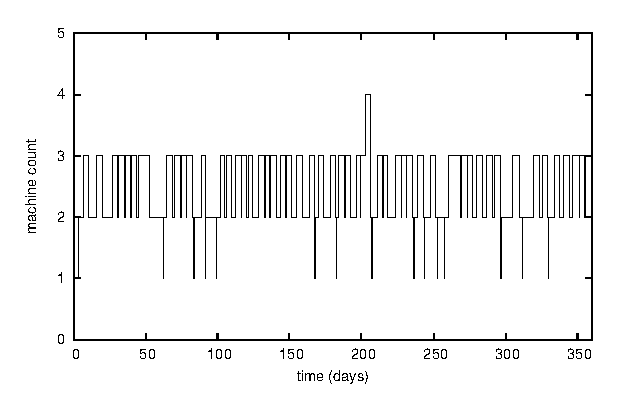
\epsfig{file=var_struct_models_figs/machine_plot.eps}
\caption{Active machine count over one year.}
\label{fig:active_machine_plot}
\end{figure}
\begin{table}[ht]
\centering
\begin{tabular}{|l|l|l|}
\hline
Seed & Maximum machine count & Annual operating cost \\ \hline
1 & 4 & \$944.05 \\ \hline
234 & 4 & \$968.58 \\ \hline
15667 & 4 & \$980.96 \\ \hline
999 & 3 & \$933.13 \\ \hline
9090133 & 4 & \$961.65 \\ \hline
6113 & 4 & \$977.33 \\ \hline
\end{tabular}
\caption{Outcomes of ten factory simulation runs.}
\label{tab:monte_carlo_outcome}
\end{table}

